\documentclass[11pt, leqno]{scrartcl}
\usepackage{polski}
\usepackage[polish]{babel}

\usepackage{graphicx, float, caption, subcaption}
\usepackage{tabularx, multirow, hyperref, enumitem}
\usepackage{listings, xcolor}
\usepackage{amsmath, amssymb}
%\usepackage{minted}

\hypersetup{
    colorlinks=true,
    linkcolor=black,
    urlcolor=black,
    citecolor=black
}

\definecolor{md-black}{rgb}{0.12, 0.12, 0.12}
\definecolor{md-teal}{rgb}{0.38, 0.79, 0.69}
\definecolor{md-mauve}{rgb}{0.76, 0.52, 0.75}
\definecolor{md-yellow}{rgb}{0.86, 0.86, 0.67}
\definecolor{md-green}{rgb}{0.13, 0.55, 0.13}
\definecolor{md-red}{rgb}{0.82, 0.10, 0.14}
\definecolor{md-purple}{rgb}{0.69, 0.33, 0.73}
\definecolor{md-orange}{rgb}{0.96, 0.42, 0.18}
\definecolor{md-gray}{rgb}{0.44, 0.46, 0.51}
\lstset{
    language=Python,
    basicstyle=\color{md-teal}\ttfamily,
    keywordstyle=\color{md-mauve},
    commentstyle=\color{md-green},
    stringstyle=\color{md-red},
    numbers=left,
    numberstyle=\small\color{md-gray}\ttfamily,
    stepnumber=1,
    numbersep=5pt,
    backgroundcolor=\color{md-black},
    showspaces=false,
    showstringspaces=false,
    showtabs=false,
    frame=none,
    tabsize=4,
    captionpos=b,
    breaklines=true,
    breakatwhitespace=false,
    escapeinside={\%*}{*)},
    numbersep=-10pt,
    morekeywords={as},
    classoffset=1,
    morekeywords={quad, quad_vec, trapz, simps, linregress,
        newton},
    keywordstyle=\color{md-yellow},
    classoffset=0
}

\graphicspath{{../images/}}

\title{Laboratorium 11 - Optymalizacja}
\author{Mateusz Podmokły - II rok Informatyka WI}
\date{6 czerwiec 2024}

\begin{document}
    \maketitle
    \section{Treść zadania}
    \textbf{Zadanie 1.} Wyznacz punkty krytyczne każdej z poniższych
    funkcji. Scharakteryzuj każdy znaleziony punkt jako minimum,
    maksimum lub punkt siodłowy. Dla każdej funkcji zbadaj, czy
    posiada minimum globalne lub maksimum globalne na zbiorze
    $\mathbb{R}^2$.
    \begin{align*}
        &f_1(x,y)=x^2-4xy+y^2 \\
        &f_2(x,y)=x^4-4xy+y^4 \\
        &f_3(x,y)=2x^3-3x^2-6xy(x-y-1) \\
        &f_4(x,y)=(x-y)^4+x^2-y^2-2x+2y+1
    \end{align*}

    \subsection*{}
    \textbf{Zadanie 2.} Należy wyznaczyć najkrótszą ścieżkę robota
    pomiędzy dwoma punktami $x^{(0)}$ i $x^{(n)}$. Problemem są
    przeszkody usytuowane na trasie robota, których należy unikać.
    Zadanie polega na minimalizacji funkcja kosztu, która sprowadza
    problem nieliniowej optymalizacji z ograniczeniami do problemu
    nieograniczonej optymalizacji. \\
    Macierz $X \in \mathbb{R}^{(n+1)\times 2}$ opisuje ścieżkę
    złożoną z $n+1$ punktów $x^{(0)},x^{(1)},x^{(2)},\ldots ,
    x^{(n)}$. Każdy punkt posiada 2 współrzędne, $x^{(i)} \in
    \mathbb{R}^2$. Punkty początkowy i końcowy ścieżki, $x^{(0)}$
    i $x^{(n)}$, są ustalone. \\
    Punkty z przeszkodami (punkty o 2 współrzędnych), $r^{(i)}$ dane
    są w macierzy przeszkód $R \in \mathbb{R}^{k\times 2}$. \\
    W celu optymalizacji ścieżki robota należy użyć metody
    największego spadku. Funkcja celu użyta do optymalizacji
    $F(x^{(0)},x^{(1)},\dots ,x^{(n)})$ zdefiniowana jest jako
    \[
        F(x^{(0)},x^{(1)},\dots ,x^{(n)})=\lambda _1
            \sum_{i=0}^{n}\sum_{j=1}^{k}\frac{1}
            {\epsilon +||x^{(i)}-r^{(j)}||_2^2}+\lambda _2
            \sum_{i=0}^{n-1}||x^{(i+1)}-x^{(i)}||_2^2
    \]
    Symbole użyte we wzorze mają następujące znaczenie:
    \begin{itemize}
        \item Stałe $\lambda _1$ i $\lambda _2$ określają wpływ
            każdego członu wyrażenia na wartość $F(X)$
            \begin{itemize}[label=--]
                \item $\lambda _1$ określa wagę składnika
                    zapobiegającego zbytniemu zbliżaniu się do
                    przeszkody,
                \item $\lambda _2$ określa wagę składnika
                    zapobiegającego tworzeniu bardzo długich
                    ścieżek,
            \end{itemize}
        \item $n$ jest liczbą odcinków, a $n+1$ liczbą punktów na
            trasie robota,
        \item $k$ jest liczbą przeszkód, których robot musi unikać,
        \item dodanie $\epsilon$ w mianowniku zapobiega dzieleniu
            przez zero.
    \end{itemize}
    \begin{enumerate}
        \item Wyprowadź wyrażenie na gradient $\nabla F$ funkcji
            celu $F$ względem $x^{(i)}$:
            \[
                \nabla F=
                \begin{bmatrix}
                    \frac{\partial F}{\partial x^{(0)}} \\
                    \vdots \\
                    \frac{\partial F}{\partial x^{(n)}}
                \end{bmatrix}
            \]
            Wzór wyraź poprzez wektory $x^{(i)}$ i ich składowe,
            wektory $r^{(i)}$ i ich składowe, $\epsilon$,
            $\lambda _1$, $\lambda _2$, $n$, i $k$ (niekoneicznie
            wszystkie). \\
            Wskazówka: $\frac{\partial ||x||^2}{\partial x}=2x$.
        \item Opisz matematycznie i zaimplementuj kroki algorytmu
            największego spadku z przeszukiwaniem liniowym, który
            służy do minimalizacji funkcji celu $F$. Do
            przeszukiwania liniowego (ang. line search) użyj metody
            złotego podziału (ang. golden section search). W tym
            celu załóż, że $F$ jest unimodalna (w rzeczywistości tak
            nie jest) i że można ustalić początkowy przedział,
            w którym znajduje się minimum.
        \item Znajdź nakrótszą ścieżkę robota przy użyciu algorytmu
            zaimplementowanego w poprzednim punktcie. Przyjmij
            następujące wartości parametrów:
            \begin{itemize}
                \item $n=20$,
                \item $k=50$,
                \item $x^{(0)}=[0,0]$,
                \item $x^{(n)}=[20,20]$,
                \item $r^{(i)}\sim \mathcal{U}(0,20)\times
                    \mathcal{U}(0,20)$,
                \item $\lambda _1=1$,
                \item $\lambda _2=1$,
                \item $\epsilon =10^{-13}$,
                \item liczba iteracji = 400.
            \end{itemize}
            Ponieważ nie chcemy zmieniać położenia punktu
            początkowego i końcowego, $x^{(0)}$ i $x^{(n)}$,
            wyzeruj gradient funkcji $F$ względem tych punktów. \\
            Obliczenia przeprowadź dla 5 różnych losowych
            inicjalizacji punktów wewnątrz ścieżki
            $x^{(1)},\ldots,x^{(n-1)}$. \\
            Narysuj przykładowy wykres wartości funkcji $F$
            w zależności od iteracji.
    \end{enumerate}

    \section{Specyfikacja użytego środowiska}
    Specyfikacja:
    \begin{itemize}
        \item Środowisko: Visual Studio Code,
        \item Język programowania: Python,
        \item System operacyjny: Microsoft Windows 11,
        \item Architektura systemu: x64.
    \end{itemize}

    \section{Rozwiązanie problemu}
    \subsection{Biblioteki}
    W realizacji rozwiązania wykorzystane zostały następujące
    biblioteki:
    \begin{lstlisting}
    import numpy as np
    import matplotlib.pyplot as plt
    \end{lstlisting}

    \subsection{Zadanie 1.}
    Punkty krytyczne zostały znalezione przy pomocny metody Newtona.
    Metoda Newtona wybiera punkt startowy $x_0$ i wykonuje kolejne
    iteracje przybliżające rozwiązanie:
    \[
        x_{k+1}=x_k-H(x_k)^{-1}\nabla f(x_k)
    \]
    gdzie $\nabla f(x,y)$ to gradient funkcji $f$ dany wzorem
    \[
        \nabla f(x,y)=
        \begin{bmatrix}
            \frac{\partial f}{\partial x}(x,y) \\
            \frac{\partial f}{\partial y}(x,y)
        \end{bmatrix}
    \]
    a $H(x,y)$ to macierz Hessego dana wzorem
    \[
        H(x,y)=
        \begin{bmatrix}
            \frac{\partial ^2f}{\partial x^2}(x,y) &
                \frac{\partial ^2f}{\partial x\partial y}(x,y) \\
            \frac{\partial ^2f}{\partial y\partial x}(x,y) &
            \frac{\partial ^2f}{\partial y^2}(x,y)
        \end{bmatrix}
    \]
    Punkt krytyczny jest minimum, jeżeli wszystkie wartości własne
    macierzy Hessego są większe od 0, maksimum jeżeli są mniejsze od
    0, a punktem siodłowym w każdej innej sytuacji. Wartości własne
    macierzy $A$ można wyznaczyć z równania
    \[
        det(A-\lambda I)=0
    \]
    gdzie $det()$ to wyznacznik macierzy, a $I$ to macierz
    jednostkowa. Do obliczenia wartości własnych wykorzystałem
    funkcję z biblioteki \texttt{NumPy}
    \[
        \texttt{np.linalg.eig}
    \]

    \subsection{Zadanie 2.}
    \subsubsection{Gradient funkcji celu}
    Na początku wyprowadzamy wzór na pochodną cząstkową funkcji
    celu $F$. \\
    Dla $i \in [1,n-1]$ mamy
    \[
        \frac{\partial F}{\partial x^{(i)}}=2\lambda _2
            (2x^{(i)}-x^{(i-1)}-x^{(i+1)})-2\lambda _1\sum_{j=1}^{k}
            \frac{x^{(i)}-r^{(j)}}{(\epsilon +
            ||x^{(i)}-r^{(j)}||^2)^2}
    \]
    dla $i \in \{ 0,n \}$
    \[
        \frac{\partial F}{\partial x^{(i)}} = (0,0)
    \]
    ponieważ chcemy, aby punkty $x_0$ oraz $x_n$ nie zmieniały
    swojego położenia.
    Zatem, gradient funkcji $F$ dany jest wzorem
    \[
        \nabla F=
        \begin{bmatrix}
            \frac{\partial F}{\partial x^{(0)}} \\
            \vdots \\
            \frac{\partial F}{\partial x^{(n)}}
        \end{bmatrix}
    \]

    \subsubsection{Algorytm największego spadku}
    Algorytm iteracyjny polega na przybliżaniu minimum zadanej
    funkcji celu $F$. Polega na wybraniu punktu początkowego
    $x_0$ i obliczaniu w kolejnych iteracjach
    \[
        x_{k+1}=x_k+\alpha _kd_k
    \]
    gdzie
    \[
        d_k=-\nabla F(x_k)
    \]
    a $\alpha _k$ to minimum funkcji $F$ wzdłuż kierunku $d_k$.
    Możemy je znaleźć metodą złotego podziału (ang. golden section
    search).

    \subsubsection{Metoda złotego podziału}
    Wybiearmy początkowe oszacowanie przedziału $[a,b]$, w naszym
    przypadku
    \[
        a=0
    \]
    \[
        b=1
    \]
    W każdej iteracji przybliżamy szukane minimum obliczając
    \[
        \alpha _1=b-\frac{b-a}{\rho}
    \]
    \[
        \alpha _2=a+\frac{b-a}{\rho}
    \]
    gdzie
    \[
        \rho =\frac{\sqrt{5}+1}{2}
    \]
    Jeżeli $f(\alpha _1)<f(\alpha _2)$ to
    \[
        b=\alpha _2
    \]
    w przeciwnym wypadku
    \[
        a=\alpha _1
    \]
    Ostateczny wynik to
    \[
        \alpha =\frac{a+b}{2}
    \]

    \section{Przedstawienie wyników}
    \subsection{Zadanie 1.}
    Zestawienie punktów krytycznych funkcji. \\
    Funkcja $f_1$:
    \begin{itemize}
        \item $(0,0)$ - punkt siodłowy, $x_0=(1,1)$
    \end{itemize}
    Funkcja $f_2$:
    \begin{itemize}
        \item $(-1,-1)$ - minimum, $x_0=(-2,-2)$
        \item $(1,1)$ - minimum, $x_0=(2,2)$
        \item $(0,0)$ - punkt siodłowy, $x_0=(-0.5,0)$
    \end{itemize}
    Funkcja $f_3$:
    \begin{itemize}
        \item $(-1,-1)$ - maksimum, $x_0=(-2,-2)$
        \item $(1,0)$ - minimum, $x_0=(2,0)$
        \item $(0,-1)$ - punkt siodłowy, $x_0=(0,-2)$
        \item $(0,0)$ - punkt siodłowy, $x_0=(0,1)$
    \end{itemize}
    Funkcja $f_4$:
    \begin{itemize}
        \item $(1,1)$ - punkt siodłowy, $x_0=(0,0)$
    \end{itemize}

    \subsection{Zadanie 2.}
    Najkrótsze ścieżki robota dla 5 losowych inicjalizacji punktów
    początkowych $x_i$ oraz $r_i$:
    \begin{figure}[H]
        \centering
        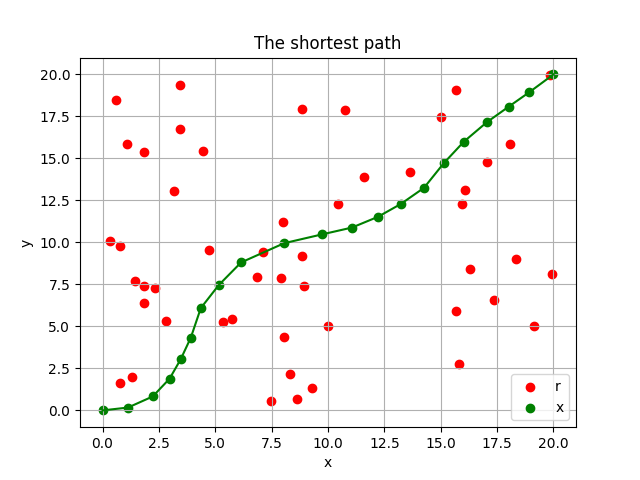
\includegraphics[width=0.7\linewidth]{path1.png}
        \caption{Ścieżka 1.}
    \end{figure}
    \begin{figure}[H]
        \centering
        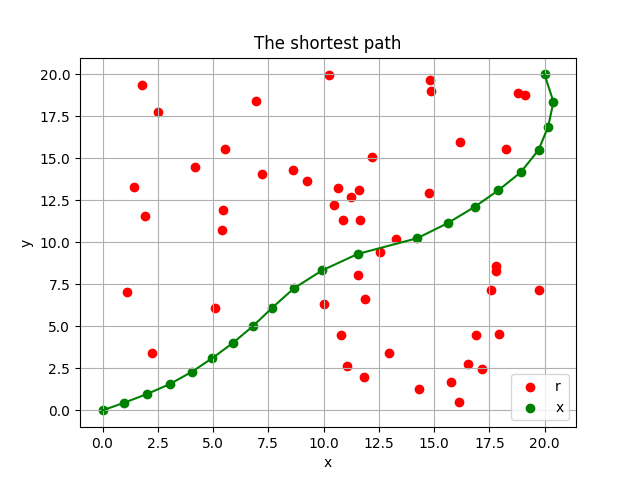
\includegraphics[width=0.7\linewidth]{path2.png}
        \caption{Ścieżka 2.}
    \end{figure}
    \begin{figure}[H]
        \centering
        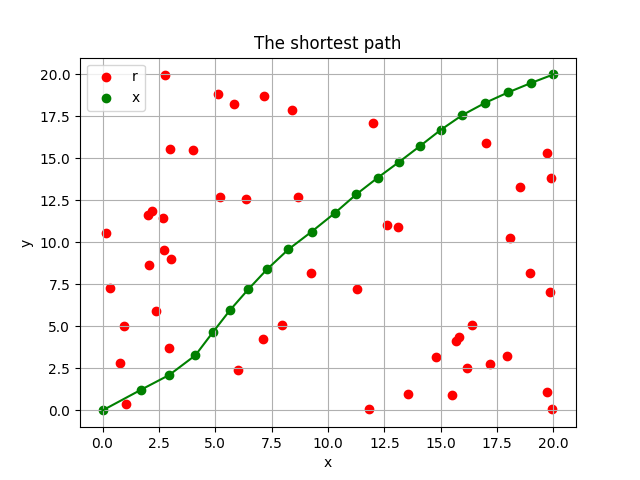
\includegraphics[width=0.7\linewidth]{path3.png}
        \caption{Ścieżka 3.}
    \end{figure}
    \begin{figure}[H]
        \centering
        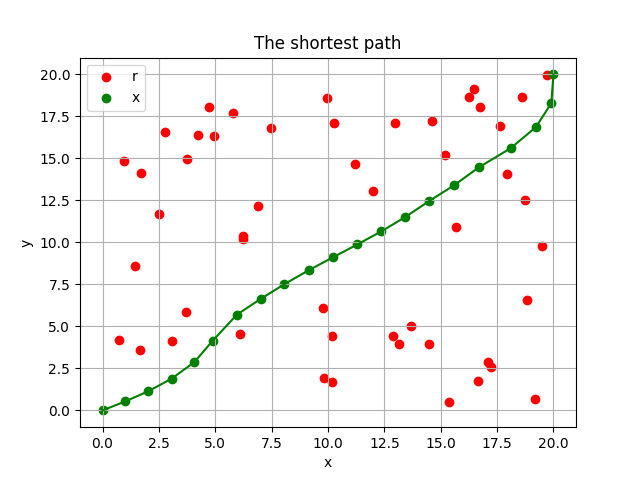
\includegraphics[width=0.7\linewidth]{path4.png}
        \caption{Ścieżka 4.}
    \end{figure}
    \begin{figure}[H]
        \centering
        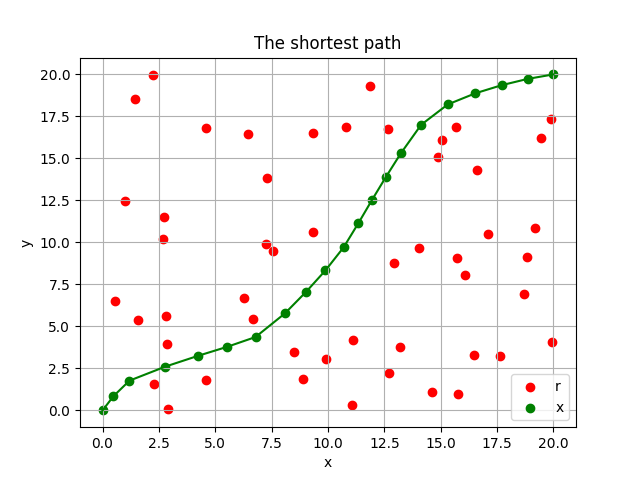
\includegraphics[width=0.7\linewidth]{path5.png}
        \caption{Ścieżka 5.}
    \end{figure}
    Przykładowy wykres wartości funkcji $F$:
    \begin{figure}[H]
        \centering
        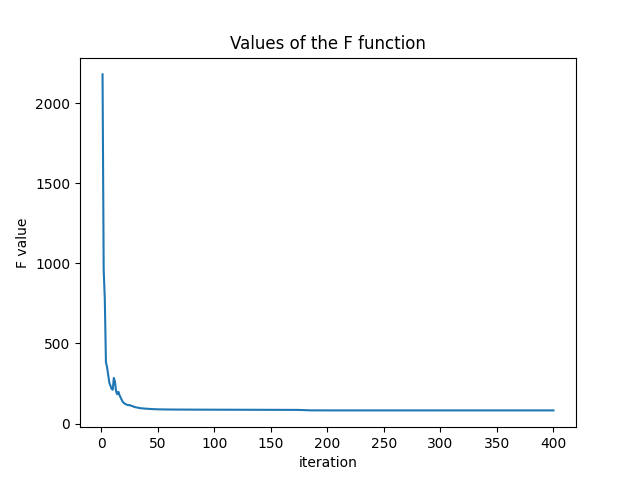
\includegraphics[width=0.7\linewidth]{F_values.png}
        \caption{Wartości funkcji $F$ w zależności od iteracji.}
    \end{figure}

    \section{Wnioski}
    Metoda Newtona jest skutecznym sposobem znajdowania punktów
    krytycznych funkcji. Powinniśmy pamiętać o odpowiednim doborze
    punktów początkowych $x_0$. \\
    Algorytm największego spadku, z wykorzystaniem metody złotego
    podziału do znajdowania minimum funkcji jednej zmiennej,
    poprawnie przybliża najmniejszą wartość funkcji celu w każdej
    iteracji. Także wymaga doboru punktu początkowego
    $x_0$, a dodatkowo, początkowego przedziału $[a,b]$ dla funkcji
    wzdłuż wektora $d$. \\
    Optymalizacja funkcji celu jest przydatnym zagadnieniem
    odpowiadającym na szeroki zakres problemów. Jednak, jak w przypadku
    wielu algorytmów numerycznych, konieczny jest odpowiedni
    dobór parametrów.

    \section{Bibliografia}
    \url{https://pl.wikipedia.org/wiki/Metoda_Newtona_
        (optymalizacja)} \\
    \url{https://pl.wikipedia.org/wiki/Metoda_najszybszego_
        spadku} \\
    \url{https://pl.wikipedia.org/wiki/Gradient_(matematyka)} \\
    \url{https://home.agh.edu.pl/~gora/algebra/Wyklad07.pdf} \\
    \url{https://pl.wikipedia.org/wiki/Macierz_Hessego} \\
    \url{https://pl.wikipedia.org/wiki/Pochodna_cz%C4%85stkowa} \\
    \url{https://pl.wikipedia.org/wiki/Metoda_z\%C5\%82otego_
        podzia\%C5\%82u}
\end{document}
